\section{System Overview of REMARK} \label{sec:system}
%
To address the two challenges raised in Sec.~\ref{sec:motivation}, this paper proposes REMARK, an efficient and reliable hybrid checkpointing framework. 

\subsection{Hybrid Checkpointing for TPC}   \label{sec:sysHybridCP}
%
As discussed above, there are three types of operations located in TPC that are executed on different devices and have different atomicity.
REMARK divides the program according the operation types into static zones and dynamic zones, as shown in Fig.~\ref{fig:InteractDefine} (a).
Static zones are constructed with I/O operations and the dynamic zones are constructed with computing operations.
Note that, the source code of a program only contains computing and I/O operations. 
All the peripheral operations are started by specific I/O operations.
Based on this division, REMARK defines three different kinds of checkpoints to recover each type of operations.

\noindent\textbf{Dynamic Checkpoint (DCP).\ \ }
%
DCPs are used to recover a computing operation by placing checkpoint exactly where power failure takes place to achieve optimal efficiency, as shown in Fig.~\ref{fig:InteractDefine} (b).
DCPs do not need to be preset in the program and are enabled only in dynamic zones.

\noindent\textbf{Static Peripheral Recover Checkpoint (SCCP).\ \ }
%
SCCPs are preset checkpoints that can restore the states of both the processor and the peripheral to re-execute an I/O operation, as shown in Fig.~\ref{fig:InteractDefine} (c).
SCCPs are set before each I/O operation in static zones where dynamic checkpoints are disabled.

\noindent\textbf{Static Peripheral Restart Checkpoint (SSCP).\ \ }
SSCPs are preset checkpoints after each I/O operation that starts a peripheral operations.
SSCP only recovers and restart the uncompleted peripheral operation and is compatible with the other two checkpoints, as shown in Fig.~\ref{fig:InteractDefine} (d).

In conclusion, with these three kinds of checkpoints, a TPC can recover all the devices and uncompleted operation reliably and efficiently. 
To realize this strategy, the REMARK has to provide hardware and software supports to establish the peripheral recovering and restarting functions for SCCP and SSCP.

%   
\begin{figure}[t]
    \centering
    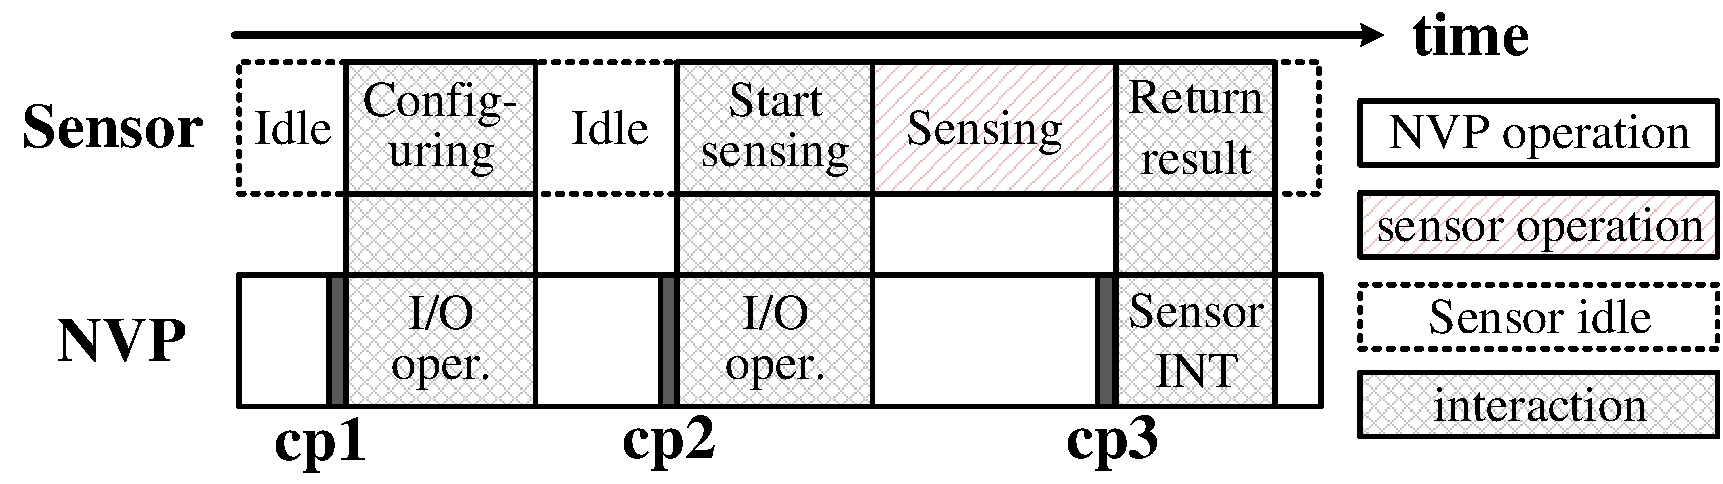
\includegraphics[width=0.48\textwidth]{Fig7_InteractDefine}
    %\vspace{-15pt}
    \caption{Interactions between processor and peripheral.}
    %\vspace{-5pt}
    \label{fig:InteractDefine}
\end{figure}

\subsection{HW/SW Architecture Support}   \label{sec:sysArch}
%
To support the hybrid checkpointing strategy, we propose a HW/SW cooperated framework to solve the two drawbacks posed by the inflexibility of NVP and inefficient recovery of peripherals, as discussed in Sec.~\ref{sec:motiHW}.
Fig.~\ref{fig:SystemArchitecture} shows the overview of REMARK framework, which contains an enhanced NVP architecture and an offline program transformer to support peripheral recovering, restarting and the two peripheral-related checkpoints.

The rest of this section presents the overview of each component.
The details will be covered in the rest of this paper. 

%\vspace{5pt}
% hardware
\noindent\textbf{Enhanced NVP Hardware Support.} \\
As shown in Fig. 4, on top of existing NVP that can instantly backup and restore the system state, REMARK adds four new modules to satisfy the requirements for flexible B/R functions and efficient peripheral recovery.

To realize flexible control of dynamic checkpointing functions, \textbf{B/R Manager} is designed based on the traditional B/R controller enabling both active and passive B/R operation.
Moreover, bootstrap is also added in this module to control the processor starting procedure.

\textbf{Peripheral State Registers (PSRs)}, \textbf{Peripheral Restart Module (PRM)} and \textbf{INT Recognizer (IRec)} are used to realize efficient and reliable peripheral recovering and restarting.
PSR is a real-time monitor storing the peripheral states to support the efficient peripheral recovering.
PRM is used to accelerates the peripheral restart procedure by automatically locating the start function in the program and correctly returning.
With the help of PRM, extra rollback of processor is removed.
Moreover, recovering the peripheral interrupts may cause consistency problem since the states in the peripherals are ruined by power failures.
To guarantee the reliability, \textbf{INT Recognizer (IRec)} is designed to place safe checkpoints when outages crash a peripheral interrupt.

To access these new modules, five new instructions are proposed as shown in Table~\ref{tab:InstrSet}.
Design details of the hardware architecture are presented in Sec.~\ref{sec:hardware} and Fig.~\ref{fig:HardwareArchitecture}.


\begin{figure*}[!htbp]
    \centering
    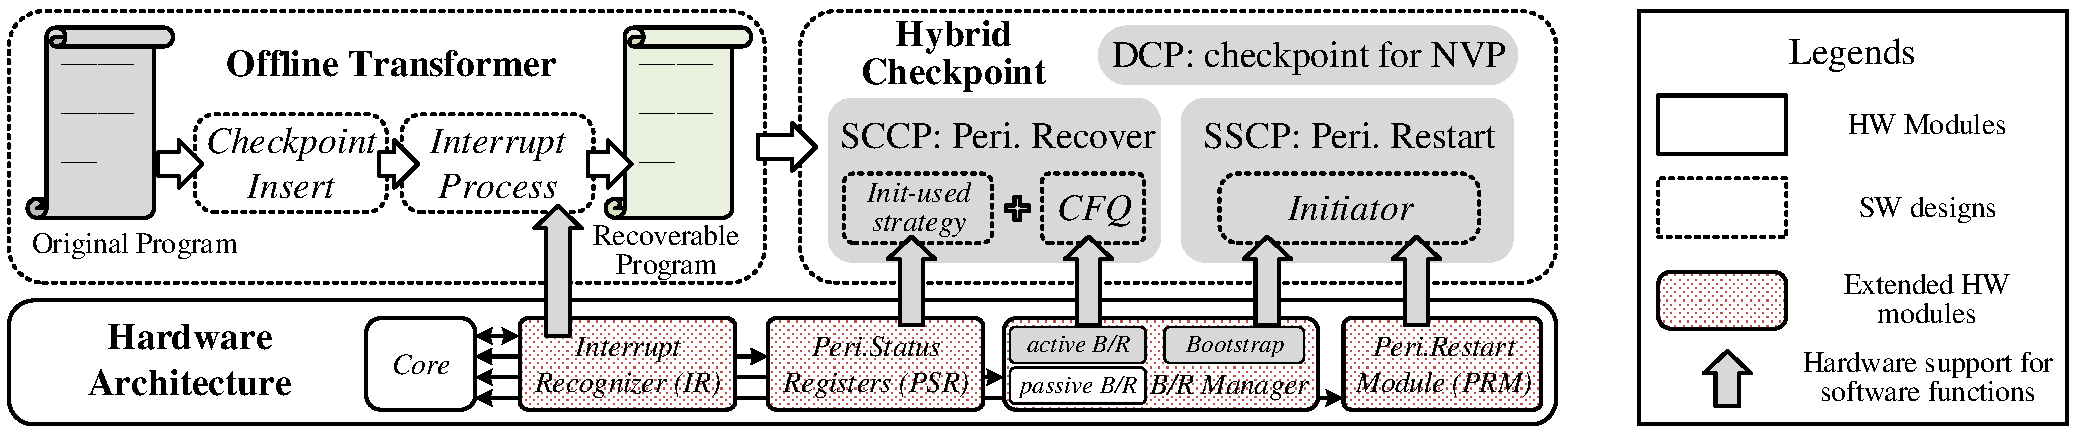
\includegraphics[width=1\textwidth]{Fig3_System.pdf}
    \caption{The HW/SW co-designed system diagram of REMARK.}
    \label{fig:SystemArchitecture}
\end{figure*}

%
\begin{figure*}[!htpb]
    \centering
    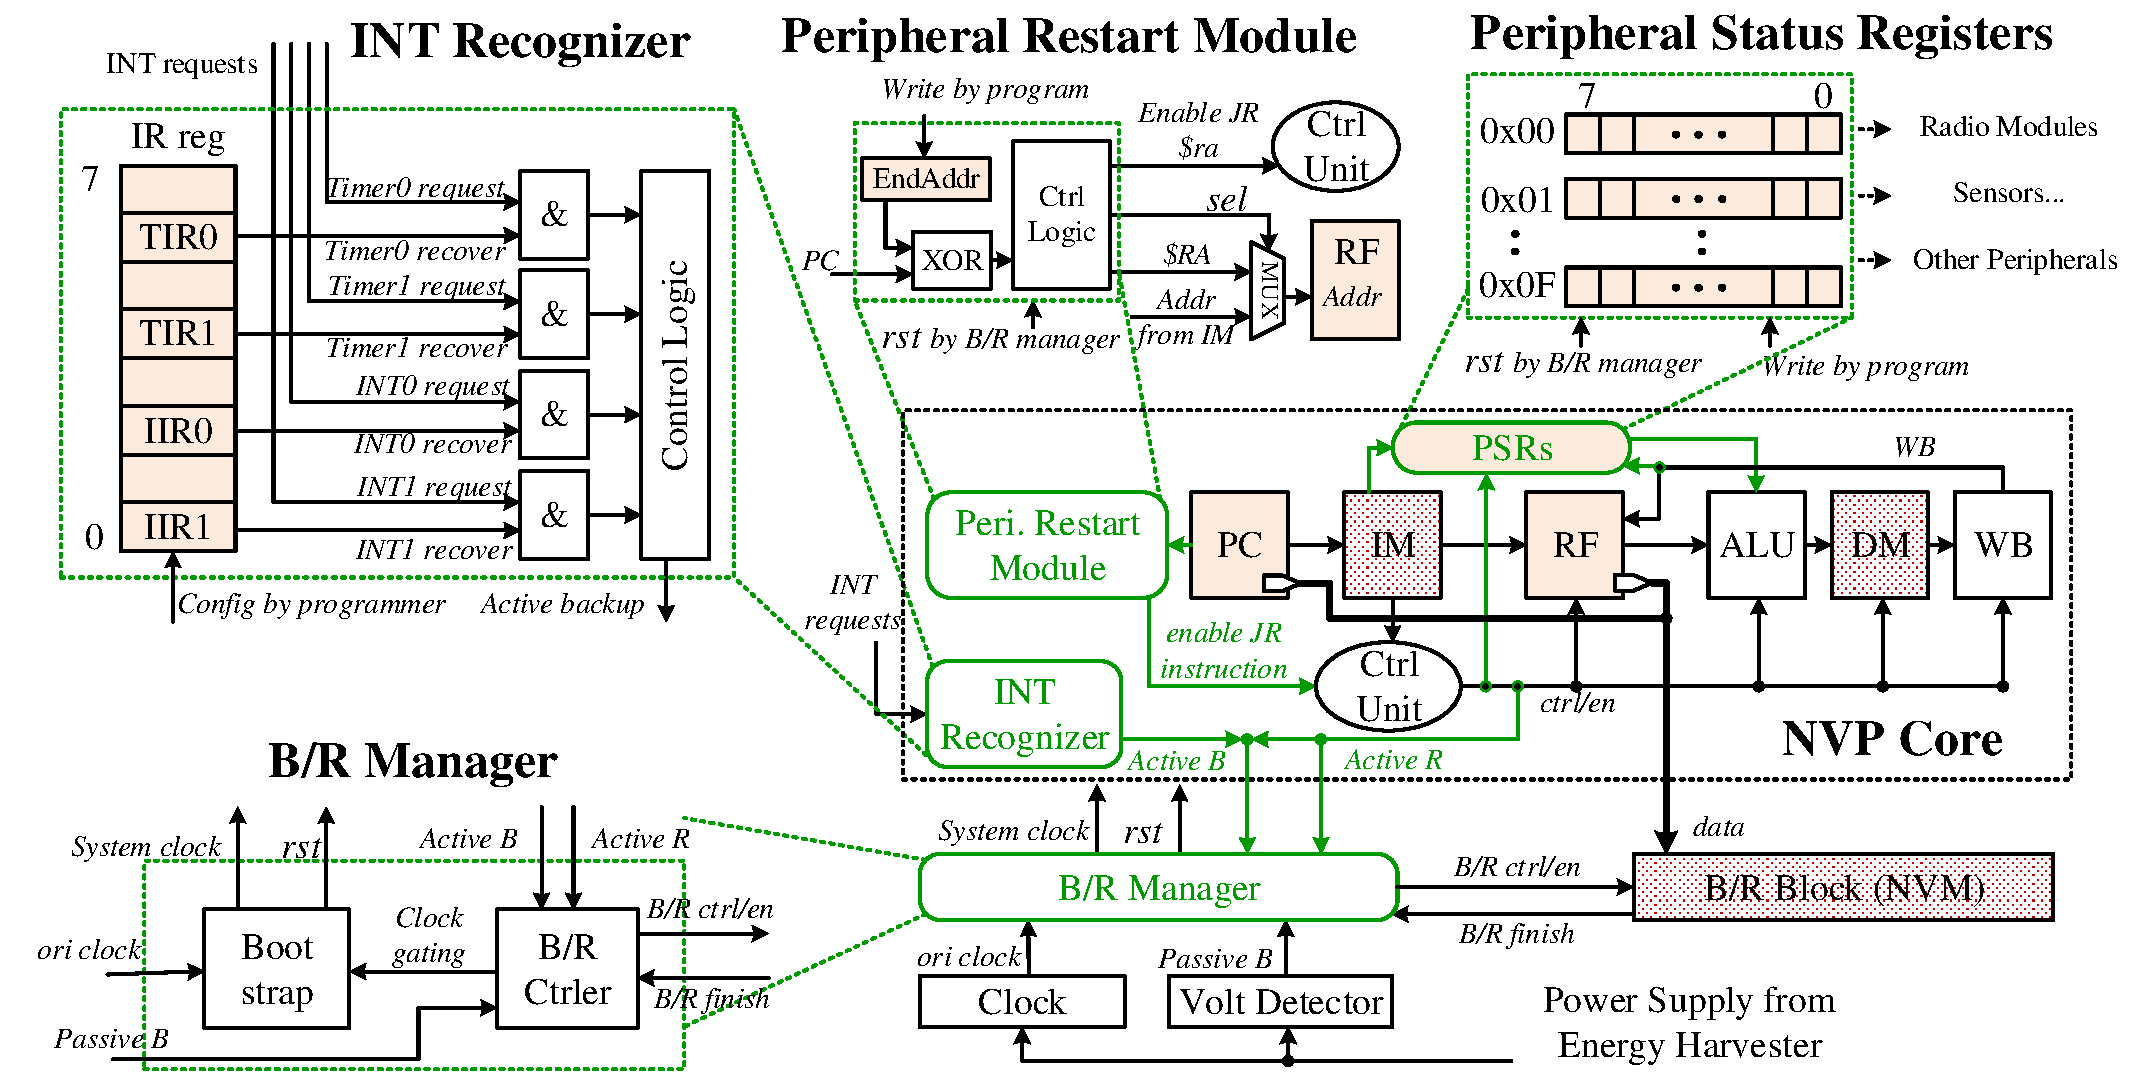
\includegraphics[width=1\textwidth]{Fig4_HardwareArchitecture.pdf}
    \caption{The hardware architecture of REMARK and its main modules. }
    \label{fig:HardwareArchitecture}
\end{figure*}

\begin{figure*}[!htbp]
    \centering
    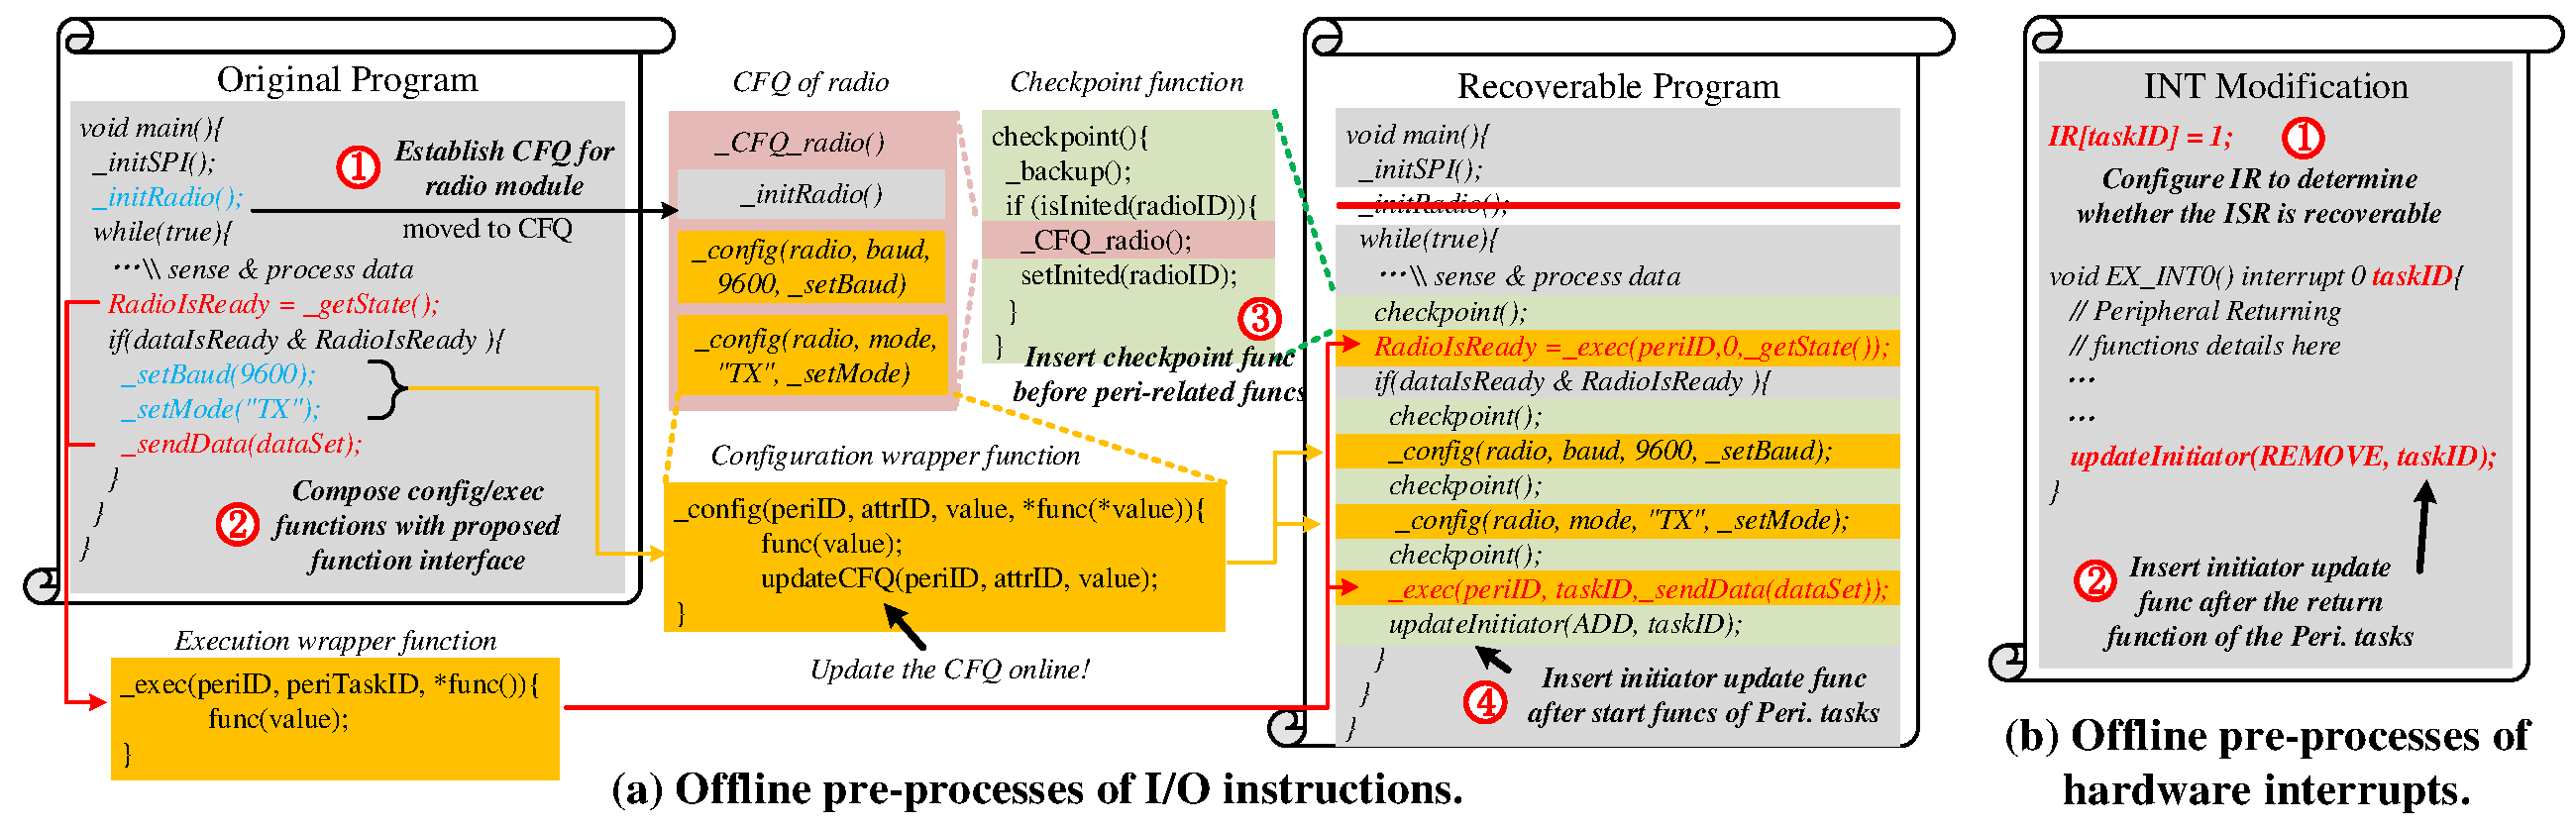
\includegraphics[width=1\textwidth]{Fig5_OfflineStage.pdf}
    \caption{The program pre-processes during the software transformation stage.}
    \label{fig:OfflineStage}
\end{figure*}


% offline
%\vspace{5pt}
\noindent\textbf{Offline Program Transformer.} \\
%
To preset the static checkpoints in the program, REMARK proposes a program transformer convert a normal program to a recoverable program where safe checkpoints are inserted as shown in Fig.\ref{fig:OfflineStage}.
APIs are provided to developers to help distinguish operations and divide the program zones.
Together with the support of the hardware framework, REMARK realizes efficient and reliable peripheral recovery and restart.
Details are presented in Sec.~\ref{sec:offline}.


% Online
%\vspace{5pt}
\begin{comment}
\noindent\textbf{Online Recover Procedure.} \\
With the support of hardware architecture and the offline program transformer, an online recover procedure is proposed containing two parts, peripheral configuration and restart.
Based on PSRs, REMARK adopts an `init-used' strategy which only initializes and configures the invoked peripherals to avoid redundant reconfiguration overheads.
A config function queue (CFQ) is used to track and stores the peripheral configuration information.
The peripheral restart is realized by Initiator where peripheral checkpoints are stored.
Initiator is supported by the bootstrap in B/R Manager to control the system restart work flow.
After power failure, Initiator restarts all the checkpointed peripherals instantly and individually.
Considering the interactions of devices, the reliability of the entire recover procedure is guaranteed by the flexible B/R functions.
Details are explained in Sec.~\ref{sec:online}.
\end{comment}

\begin{table}[t]
\caption{The extended instructions to the instruction set.}\label{tab:InstrSet}
\Fsize{8}
\renewcommand{\arraystretch}{1.5}
\begin{tabular}{cIcIm{4.4cm}}
    \Xhline{1.2pt}
    Instructions       & Operators           & Specifications      \\
    \Xhline{1pt}
    RSR      & SRaddr   oper2 & Read PSRs with address \emph{SRaddr} to register \emph{oper2}.\\
    \Xhline{1pt}
    WSR     & oper1   SRaddr & Write the value of \emph{oper1} to PSRs with address \emph{SRaddr}.\\
    \Xhline{1pt}
    WER    & oper1               & Write the value of \emph{oper1} to \emph{EndAddr} register in PRM.\\
    \Xhline{1pt}
    ABR     & oper1               & Enable the active backup function, if $oper1=1$; enable the active restore function, if $oper2=0$.\\
    \Xhline{1pt}
    EBR     & oper1               & Enable/Disable the backup and restore function when $oper1=1/oper1=0$.\\
    \Xhline{1.2pt}
\end{tabular}
\end{table}


